%%%%%%%%%%%%%%%%%%%%%%%%%%%%%%%%%%%%
% スライドオプション
%%%%%%%%%%%%%%%%%%%%%%%%%%%%%%%%%%%%

% オプション1：解答あり（授業用）

\documentclass[slidestop,compress,mathserif]{beamer}
\newcommand{\soln}[1]{\textit{#1}}
\newcommand{\solnGr}[1]{#1}

% オプション2：解答なし（配布用ハンドアウト）

%\documentclass[11pt,containsverbatim,handout]{beamer}
%\usepackage{pgfpages}
%\pgfpagesuselayout{4 on 1}[letterpaper,landscape,border shrink=5mm]
%\newcommand{\soln}[1]{ }
%\newcommand{\solnGr}{ }

%%%%%%%%%%%%%%%%%%%%%%%%%%%%%%%%%%%%
% 日本語サポート（LuaLaTeX使用）
% コンパイルコマンド: lualatex chp1.tex
%%%%%%%%%%%%%%%%%%%%%%%%%%%%%%%%%%%%

\usepackage{luatexja}
\usepackage{luatexja-fontspec}

%%%%%%%%%%%%%%%%%%%%%%%%%%%%%%%%%%%%
% スタイル
%%%%%%%%%%%%%%%%%%%%%%%%%%%%%%%%%%%%

\input{../lec_style_JP}


%%%%%%%%%%%%%%%%%%%%%%%%%%%%%%%%%%%%
% プリアンブル
%%%%%%%%%%%%%%%%%%%%%%%%%%%%%%%%%%%%

\title[第1章：データ入門]{第1章：データ入門}
\author{OpenIntro Statistics 第4版（日本語版）}
\institute{$\:$ \\ {\footnotesize 原著スライド：Mine \c{C}etinkaya-Rundel（OpenIntro）\\
\webLink{http://creativecommons.org/licenses/by-sa/3.0/us/}{CC BY-SA ライセンス}のもと使用・翻訳。\\
一部の画像はフェアユース（教育目的）に基づき使用。}}
\date{}

%%%%%%%%%%%%%%%%%%%%%%%%%%%%%%%%%%%%
% ドキュメント開始
%%%%%%%%%%%%%%%%%%%%%%%%%%%%%%%%%%%%

\begin{document}


%%%%%%%%%%%%%%%%%%%%%%%%%%%%%%%%%%%%
% タイトルページ
%%%%%%%%%%%%%%%%%%%%%%%%%%%%%%%%%%%%

{
\addtocounter{framenumber}{-1}
{\removepagenumbers
\usebackgroundtemplate{
\includegraphics[width=\paperwidth]{../OpenIntro_Grid_4_3-01.jpg}}
\begin{frame}

\hfill 
\includegraphics[width=20mm]{../oiLogo_highres}

\titlepage

\end{frame}
}
}


%%%%%%%%%%%%%%%%%%%%%%%%%%%%%%%%%%%%
% 各節
%%%%%%%%%%%%%%%%%%%%%%%%%%%%%%%%%%%%

%%%%%%%%%%%%%%%%%%%%%%%%%%%%%%%%%%%%

\section{ケーススタディ}

%%%%%%%%%%%%%%%%%%%%%%%%%%%%%%%%%%%%

\begin{frame}
\frametitle{慢性疲労症候群の治療}

\begin{itemize}

\item \textbf{目的：}慢性疲労症候群に対する認知行動療法の効果を評価する。

\item \textbf{参加者候補：}かかりつけ医や専門医から慢性疲労症候群専門クリニックへ紹介された142名の患者。

\item \textbf{実際の参加者：}紹介された142名のうち、実際に研究へ参加したのは60名のみ。
診断基準を満たさない者、他の健康上の問題を抱える者、参加を拒否した者は除外された。

\end{itemize}

\ct{Deale et. al. \textit{Cognitive behavior therapy for chronic fatigue syndrome: A randomized controlled trial}. The American Journal of Psychiatry 154.3 (1997).}

\end{frame}

%%%%%%%%%%%%%%%%%%%%%%%%%%%%%%%%%%%%

\begin{frame}
\frametitle{研究デザイン}

\begin{itemize}

\item 患者は治療群と対照群にランダムに割り当てられ、各群30名：
\begin{itemize}
\item \hl{治療群}：認知行動療法――協調的・教育的なアプローチで行動面を重視。
症状を悪化させることなく活動量を段階的・安全に増やす方法を患者に指導した。
\item \hl{対照群}：リラクゼーション――活動量を増やす指導は行わず、
筋弛緩法・視覚化・即時リラクゼーション技法を指導した。
\end{itemize}

\end{itemize}

\end{frame}

%%%%%%%%%%%%%%%%%%%%%%%%%%%%%%%%%%%%

\begin{frame}
\frametitle{結果}

下の表は、6か月後の追跡調査における良好な転帰を示した患者の分布を示す。
なお、7名（治療群3名・対照群4名）が途中で脱落した。

\begin{center}
\begin{tabular}{ll  cc c}
			&				& \multicolumn{2}{c}{\textit{良好な転帰}} \\
\cline{3-4}
			&							& あり 	& なし 	& 合計	\\
\cline{2-5}
						&治療群 	& 19	 	& 8		& 27 	\\
\raisebox{1.5ex}[0pt]{\textit{群}}	&対照群		& 5	 	& 21	 	& 26 \\
\cline{2-5}
						&合計		& 24		& 29		& 53
\end{tabular}
\end{center}

\begin{itemize}

\item 治療群における良好な転帰の割合：
\[ 19 / 27 \approx 0.70 \rightarrow 70\% \]

\item 対照群における良好な転帰の割合：
\[ 5 / 26 \approx 0.19 \rightarrow 19\% \]

\end{itemize}

\end{frame}

%%%%%%%%%%%%%%%%%%%%%%%%%%%%%%%%%%%%

\begin{frame}
\frametitle{結果の解釈}

\dq{データはグループ間の「真の」差を示しているか？}

\begin{itemize}

\item コインを100回投げることを考えてみよう。
表が出る確率は50\%だが、ちょうど50回表が出るとは限らない。
このようなばらつきは、ほぼあらゆるデータ生成プロセスで生じる。

\item 2グループ間で観測された差（70 - 19 = 51\%）は真の差かもしれないし、
自然なばらつきによるものかもしれない。

\item 差が非常に大きいため、真の差である可能性が高いと考えられる。

\item この差が偶然によるものでないと判断できるかどうかは、統計的手法を用いて判断する必要がある。

\end{itemize}

\end{frame}

%%%%%%%%%%%%%%%%%%%%%%%%%%%%%%%%%%%%

\begin{frame}
\frametitle{結果の一般化}

\dq{この研究の結果は、慢性疲労症候群の患者全体に一般化できるか？}

これらの患者は特定の特性を持ち、自ら参加を希望した者たちであるため、
慢性疲労症候群の患者全体を代表しているとは言い難い。
ただちに全患者に一般化することはできないが、
この最初の研究は有望な結果を示している。
特定の特性を持つ患者には効果があることが示されており、
他の患者にも少なからず効果が期待できる。

\end{frame}

%%%%%%%%%%%%%%%%%%%%%%%%%%%%%%%%%%%%

%%%%%%%%%%%%%%%%%%%%%%%%%%%%%%%%%%%%

\section{データの基礎}

%%%%%%%%%%%%%%%%%%%%%%%%%%%%%%%%%%%%

\subsection{観測値と変数}

\begin{frame}
\frametitle{クラスでのアンケート}

入門統計学の受講生を対象にアンケートが実施された。
以下はアンケートの質問の一部と、それに対応する変数名である：

\begin{itemize}
\item \var{gender}：あなたの性別は？
\item \var{intro\_extra}：自分を内向的・外向的、どちらだと思いますか？
\item \var{sleep}：平均して1日何時間寝ますか？
\item \var{bedtime}：ふだん何時頃就寝しますか？
\item \var{countries}：今までに何カ国訪れたことがありますか？
\item \var{dread}：この授業への「うんざり度」を1〜5で表すと？
\end{itemize}

\end{frame}

%%%%%%%%%%%%%%%%%%%%%%%%%%%%%%%%%%%%

\begin{frame}
\frametitle{データ行列}

統計学の受講生から様々な変数についてデータを収集した：

\begin{center}
\begin{tabular}{l cccc l}
		& \hl{変数} \\
		& \hl{$\downarrow$}	 \\
\cline{1-5}
学生	&	\var{gender}	&	\var{intro\_extra} & $\cdots$ & \var{dread} \\
\cline{1-5}
1 & male   & extravert  & $\cdots$  & 3 \\
2 & female & extravert  & $\cdots$  & 2 \\
3 & female & introvert  & $\cdots$  & 4 & \hl{$\leftarrow$}  \\
4 & female & extravert  & $\cdots$  & 2 & \hl{観測値} \\
$\vdots$	 &	$\vdots$	&	$\vdots$  &	$\vdots$ &	$\vdots$ \\
86	& male & extravert  & $\cdots$  & 3 \\
\cline{1-5}
\end{tabular}
\end{center}

\end{frame}

%%%%%%%%%%%%%%%%%%%%%%%%%%%%%%%%%%%%

\subsection{変数の種類}

\begin{frame}
\frametitle{変数の種類}

\begin{center}
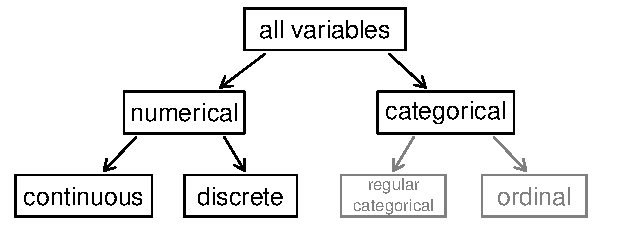
\includegraphics[width=0.9\textwidth]{1-2_data_basics/figures/variables/variables}
\end{center}

\end{frame}

%%%%%%%%%%%%%%%%%%%%%%%%%%%%%%%%%%%

\begin{frame}
\frametitle{変数の種類（続き）}

\begin{center}
{\footnotesize
\begin{tabular}{c ccc cc}
  \hline
 & \var{gender} & \var{sleep} & \var{bedtime} & \var{countries} & \var{dread} \\
  \hline
1 & male & 5 & 12-2 & 13 & 3 \\
  2 & female & 7 & 10-12 & 7 & 2 \\
  3 & female & 5.5 & 12-2 & 1 & 4 \\
  4 & female & 7 & 12-2 &  & 2 \\
  5 & female & 3 & 12-2 & 1 & 3 \\
  6 & female & 3 & 12-2 & 9 & 4 \\
  \hline
\end{tabular}
}
\end{center}

\begin{itemize}
\item \var{gender}：\soln{カテゴリ変数}
\item \var{sleep}：\soln{数値変数・連続}
\item \var{bedtime}：\soln{カテゴリ変数・順序}
\item \var{countries}：\soln{数値変数・離散}
\item \var{dread}：\soln{カテゴリ変数・順序尺度（数値変数として扱うことも可）}
\end{itemize}

\end{frame}

%%%%%%%%%%%%%%%%%%%%%%%%%%%%%%%%%%%

\begin{frame}
\frametitle{練習問題}

\pq{電話の市外局番はどのタイプの変数か？}

\begin{enumerate}[(a)]
\item 数値変数・連続
\item 数値変数・離散
\solnMult{カテゴリ変数}
\item カテゴリ変数・順序
\end{enumerate}

\end{frame}

%%%%%%%%%%%%%%%%%%%%%%%%%%%%%%%%%%%

\subsection{変数間の関係}

%%%%%%%%%%%%%%%%%%%%%%%%%%%%%%%%%%%

\begin{frame}
\frametitle{変数間の関係}

\dq{GPAと週の学習時間に関係はあるか？}

\begin{center}
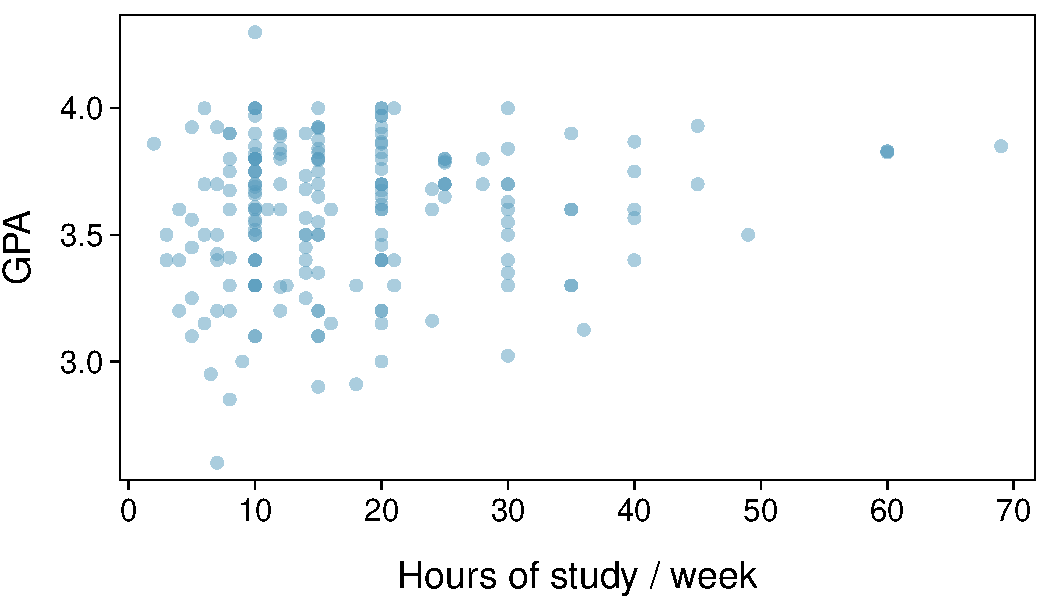
\includegraphics[width=0.7\textwidth]{1-2_data_basics/figures/gpa_study_hours/gpa_study_hours}
\end{center}

\dq{データ点に何か異常はないか？}

\soln{GPA$>$4.0の学生が1名おり、これはおそらくデータエラーである。}

\end{frame}

%%%%%%%%%%%%%%%%%%%%%%%%%%%%%%%%%%%

\subsection{説明変数と応答変数}

%%%%%%%%%%%%%%%%%%%%%%%%%%%%%%%%%%%

\begin{frame}
\frametitle{説明変数と応答変数}

\begin{itemize}

\item 2つの変数の組において説明変数を特定するには、
どちらがもう一方に影響を与えると考えられるかを判断する：

\begin{center}
説明変数 $\xrightarrow{\text{影響する可能性}}$ 応答変数
\end{center}

\item 変数を説明変数・応答変数と名付けても、
2変数間の関係が実際に因果関係であることを保証するわけではない。
関連が確認された場合でも同様である。
これらのラベルは、どちらがもう一方に影響を与えると予想されるかを
追跡するためだけに使う。

\end{itemize}

\end{frame}

%%%%%%%%%%%%%%%%%%%%%%%%%%%%%%%%%%%

\subsection{観察研究と実験の導入}

%%%%%%%%%%%%%%%%%%%%%%%%%%%%%%%%%%%

\begin{frame}
\frametitle{データ収集の2つの主要な方法}

\begin{itemize}

\item \hl{観察研究：}データが生じる過程に直接介入しない方法でデータを収集する（例：調査）。
\begin{itemize}
\item 変数間に自然に生じる関連の証拠を得ることはできるが、
それだけで因果関係を示すことはできない。
\end{itemize}

\item \hl{実験：}研究者が被験者をさまざまな処置にランダムに割り当て、
説明変数と応答変数の因果関係を確立する。

\end{itemize}

\end{frame}

%%%%%%%%%%%%%%%%%%%%%%%%%%%%%%%%%%%

\begin{frame}
\frametitle{相関と因果関係}

\begin{itemize}

\item 2つの変数が何らかの関係を示すとき、それらを\hl{関連した}変数と呼ぶ。
\begin{itemize}
\item 関連した変数は\hl{従属}変数とも呼ばれる。
\end{itemize}

\item 2つの変数が関連していない、すなわち明らかなつながりがない場合、
それらは\hl{独立}であると言う。

\item 一般に、\textbf{相関は因果関係を意味しない}。
因果関係はランダム化実験からのみ推論できる。

\end{itemize}

\begin{center}

\includegraphics[width=0.55\textwidth]{1-2_data_basics/figures/xkcd_correlation} \\
{\tiny \webURL{http://xkcd.com/552/}}
\end{center}

\end{frame}

%%%%%%%%%%%%%%%%%%%%%%%%%%%%%%%%%%%%

\begin{frame}
\frametitle{練習問題}

\twocol{0.5}{0.5}
{
\pq{右の散布図に基づき、フクロモモンガの頭の長さと頭蓋骨の幅について正しい記述はどれか？}
}
{
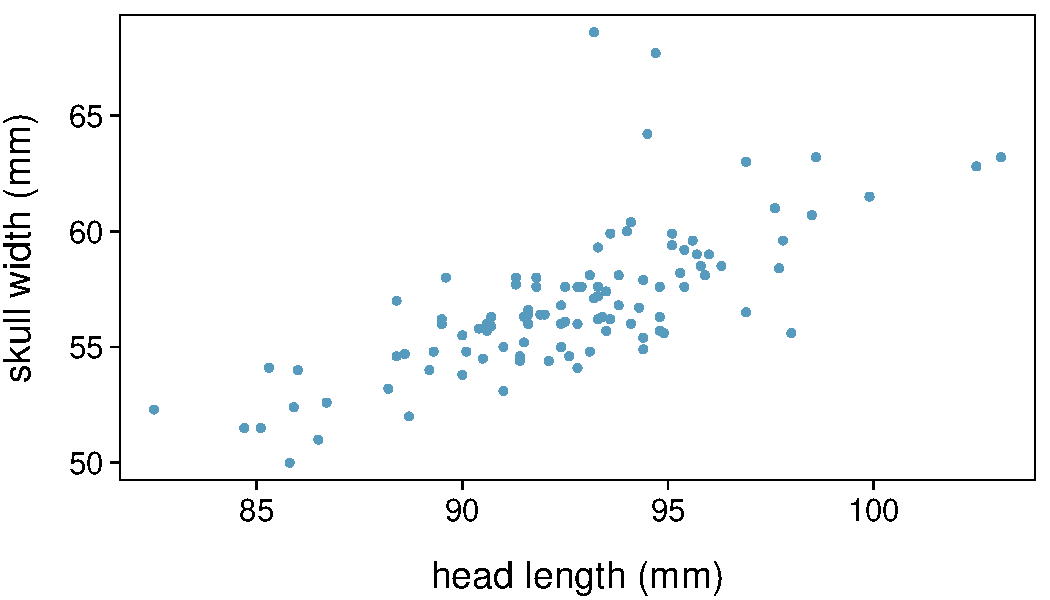
\includegraphics[width=\textwidth]{1-2_data_basics/figures/possum_head_skull/possum_head_skull}
}

\begin{enumerate}[(a)]
\item 頭の長さと頭蓋骨の幅に関係はなく、独立している。
\solnMult{頭の長さと頭蓋骨の幅は正の関連がある。}
\item 頭蓋骨の幅と頭の長さは負の関連がある。
\item 頭が長いほど頭蓋骨が広くなる（因果関係）。
\item 頭蓋骨が広いほど頭が長くなる（因果関係）。
\end{enumerate}

\end{frame}

%%%%%%%%%%%%%%%%%%%%%%%%%%%%%%%%%%%

%%%%%%%%%%%%%%%%%%%%%%%%%%%%%%%%%%%%

\section{標本抽出の原則と方法}

%%%%%%%%%%%%%%%%%%%%%%%%%%%%%%%%%%%%

\subsection{母集団と標本}

%%%%%%%%%%%%%%%%%%%%%%%%%%%%%%%%%%%%

\begin{frame}
\frametitle{母集団と標本}

\twocol{0.5}{0.5}{
\begin{center}
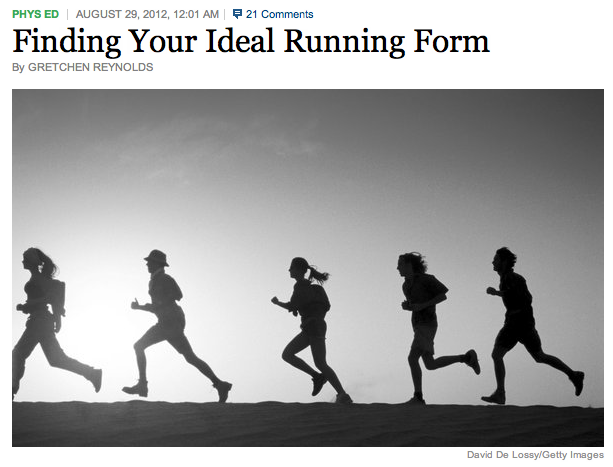
\includegraphics[width=\textwidth]{1-3_sampling_principles_strategies/figures/running}
\end{center}
\vspace{-0.5cm}
{\tiny \webURL{http://well.blogs.nytimes.com/2012/08/29/finding-your-ideal-running-form}}
}
{
\hl{研究の問い：}走ることだけで、より効率的なランナーになれるか？\\

\hl{対象母集団：}\soln{すべての人}
}
$\:$ \\
\hl{標本：}最近ランニンググループに参加した成人女性のグループ

\hl{結果を一般化できる母集団：}\soln{データがランダムにサンプリングされていれば成人女性}

\end{frame}

%%%%%%%%%%%%%%%%%%%%%%%%%%%%%%%%%%%%

\subsection{逸話的証拠}

%%%%%%%%%%%%%%%%%%%%%%%%%%%%%%%%%%%%

\begin{frame}
\frametitle{逸話的証拠と喫煙研究の黎明期}

\begin{itemize}

\item 禁煙研究は1930〜40年代、タバコの喫煙が急増した頃に始まった。
タバコの煙に敏感な喫煙者がいる一方、まったく影響を受けないように見える喫煙者もいた。

\item 禁煙研究は「私の叔父は一日3箱吸っているが至って健康だ」というような
\hl{逸話的証拠}（限られた標本に基づく根拠で、母集団を代表しない可能性がある）
に基づく反論に直面した。

\item 「喫煙は複雑な人間行動であり、その性質上研究しにくく、
個人差によって交絡されている」という結論が出された。

\item やがて研究者たちがより大きな標本（喫煙者）を検討できるようになると、
喫煙が健康に悪影響を及ぼすという傾向がはっきりと見えるようになった。

\end{itemize}

\ct{Brandt, \textit{The Cigarette Century} (2009), Basic Books.}

\end{frame}

%%%%%%%%%%%%%%%%%%%%%%%%%%%%%%%%%%%%

\subsection{母集団からの標本抽出}

%%%%%%%%%%%%%%%%%%%%%%%%%%%%%%%%%%%%

\begin{frame}
\frametitle{全数調査}

\begin{itemize}

\item 全員を対象にして、母集団全体を「サンプリング」した方がよいのではないか？
\begin{itemize}
\item これを\hl{全数調査}という。
\end{itemize}

\item 全数調査には以下のような問題がある：

\begin{itemize}
\item 全員を調査するのは難しい：見つけにくい個人や測定しにくい個人は常に存在する。
\textit{しかも、そのような見つけにくい人々は、他の人々と異なる特性を持っている可能性がある。}
\item 母集団は変化し続ける。全数調査ができたとしても、
母集団は常に変化するため、完全な測定は不可能である。
\item 全数調査は標本抽出より複雑になる場合がある。
\end{itemize}

\end{itemize}

\end{frame}

%%%%%%%%%%%%%%%%%%%%%%%%%%%%%%%%%%%%%

\begin{frame}

\vfill

\begin{center}
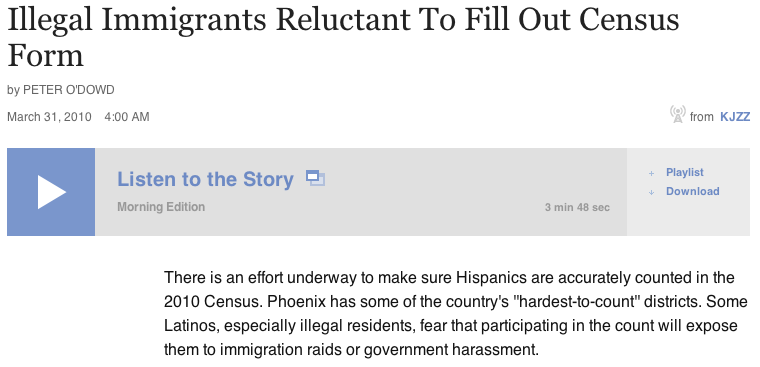
\includegraphics[width=0.90\textwidth]{1-3_sampling_principles_strategies/figures/census_illegal_immig}
\end{center}

\ct{\webURL{http://www.npr.org/templates/story/story.php?storyId=125380052}}

\end{frame}

%%%%%%%%%%%%%%%%%%%%%%%%%%%%%%%%%%%%%

\begin{frame}
\frametitle{探索的分析から推測へ}

\begin{itemize}

\item 標本抽出は自然な営みである。

\item 料理中の食べ物を味見することを考えてみよう――料理全体の味を知るために、
その一部（標本）を味見（検査）する。

\item スープを一口味見して「塩気が足りない」と思うのが\hl{探索的分析}である。

\item そこから「スープ全体に塩が足りない」と結論づけるのが\hl{推測}である。

\item 推測が有効であるためには、味見した一口（標本）が鍋全体（母集団）を
\hl{代表している}必要がある。

\begin{itemize}
\item 表面からしか取っていない一口が、塩が底に溜まっているスープを代表しているとは言えない。
\item よくかき混ぜてから味見すれば、一口はスープ全体を代表しやすくなる。
\end{itemize}

\end{itemize}

\end{frame}

%%%%%%%%%%%%%%%%%%%%%%%%%%%%%%%%%%%%

\begin{frame}
\frametitle{標本バイアス}

\begin{itemize}

\item \hl{無回答バイアス：}ランダムにサンプリングされた人のうちごく一部しか
調査に回答しない場合、標本はもはや母集団を代表していない可能性がある。

\item \hl{自発的回答バイアス：}その問題について強い意見を持つ人が
自ら進んで回答することで標本が構成される場合。
このような標本も母集団を代表しない。

\begin{center}

\includegraphics[width=0.25\textwidth]{1-3_sampling_principles_strategies/figures/vol_resp_bias/vol_resp_bias_q}
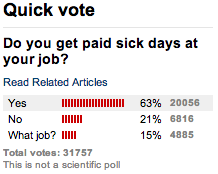
\includegraphics[width=0.25\textwidth]{1-3_sampling_principles_strategies/figures/vol_resp_bias/vol_resp_bias_res} \\
{\tiny cnn.com, 2012年1月14日}
\end{center}

\item \hl{便宜的標本：}アクセスしやすい個人が標本に含まれやすくなる。

\end{itemize}

\end{frame}

%%%%%%%%%%%%%%%%%%%%%%%%%%%%%%%%%%%%

\begin{frame}
\frametitle{標本バイアスの例：ランドン対FDR}

偏った標本が誤った結果をもたらした歴史的な例：\\

$\:$ \\

\begin{columns}[c]

\column{0.35\textwidth}

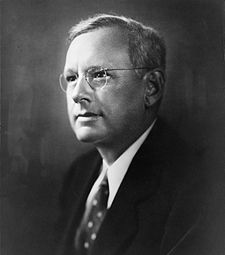
\includegraphics[width= \textwidth]{1-3_sampling_principles_strategies/figures/landon_fdr/landon}

\column{0.3\textwidth}
1936年、ランドンはFDR（フランクリン・ルーズベルト）の再選に対抗して
共和党の大統領候補を目指した。

\column{0.35\textwidth}

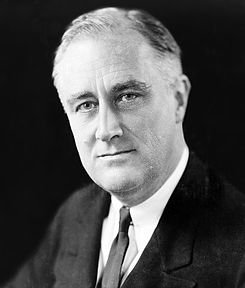
\includegraphics[width= \textwidth]{1-3_sampling_principles_strategies/figures/landon_fdr/fdr}

\end{columns}

\end{frame}

%%%%%%%%%%%%%%%%%%%%%%%%%%%%%%%%%%%%%

\begin{frame}
\frametitle{リテラリー・ダイジェスト誌の世論調査}

\begin{columns}

\column{0.7\textwidth}

\begin{itemize}

\item リテラリー・ダイジェスト誌は約1,000万人のアメリカ人に調査を行い、
約240万人から回答を得た。

\item 調査ではランドンが圧勝し、FDRの得票率は43\%にとどまると予測された。

\item 実際の選挙結果：FDRが62\%の票を獲得して勝利した。

\end{itemize}

\column{0.3\textwidth}

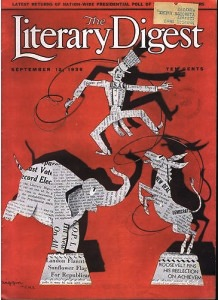
\includegraphics[width= \textwidth]{1-3_sampling_principles_strategies/figures/literaryDigest}

\end{columns}

\begin{itemize}

\item この雑誌は世論調査の失敗によって信頼を完全に失い、まもなく廃刊となった。

\end{itemize}

\end{frame}

%%%%%%%%%%%%%%%%%%%%%%%%%%%%%%%%%%%%%

\begin{frame}
\frametitle{リテラリー・ダイジェスト誌の世論調査――何が間違っていたか？}

\begin{itemize}

\item この雑誌が調査対象としたのは、

\begin{itemize}

\item 自誌の読者、

\item 自動車の登録者、そして

\item 電話の契約者であった。

\end{itemize}

\item これらのグループは当時（大恐慌の時代であることを思い出してほしい）の
全国平均を大きく上回る収入を持っており、
共和党を支持する有権者が多く含まれていた。
つまり標本は当時のアメリカの\hl{典型的な}有権者を代表していなかった。

\end{itemize}

\end{frame}

%%%%%%%%%%%%%%%%%%%%%%%%%%%%%%%%%%%%%

\begin{frame}
\frametitle{大きな標本は望ましいが……}

\begin{itemize}

\item リテラリー・ダイジェスト誌の世論調査は240万人という巨大な標本に基づいていたが、
標本に\hl{バイアス}があったため、正確な予測はできなかった。

\item スープの例えに戻ると：
スープがよくかき混ぜられていなければ、スプーンがいくら大きくても味は正しく分からない。
よくかき混ぜてあれば、小さなスプーンで十分である。

\end{itemize}

\end{frame}

%%%%%%%%%%%%%%%%%%%%%%%%%%%%%%%%%%%%%

\begin{frame}[shrink]
\frametitle{練習問題}

{\small
\pq{ある学区が、最近2件の生徒の重傷事故を受けて、高校生の校内駐車を禁止するか
検討している。最初の一歩として、保護者に郵送でアンケートを行い、
この方針変更に反対するかどうかを尋ねた。送付した6,000通のうち、
返送されたのは1,200通であった。回答のあった1,200通のうち、960通が方針変更に賛成、
240通が反対であった。次の記述のうち正しいものはどれか？}

\begin{enumerate}[I.]
\item 郵便物が保護者に届かなかった可能性がある。
\item 学区は方針変更について保護者から強い支持を得ている。
\item 高校生の保護者の多数が方針変更に反対している可能性がある。
\item すべての保護者に調査票を送ったのだから、調査結果にバイアスが生じる可能性は低い。
\end{enumerate}

\begin{multicols}{5}
\begin{enumerate}[(a)]
\item Iのみ
\item IとII
\solnMult{IとIII}
\item IIIとIV
\item IVのみ
\end{enumerate}
\end{multicols}
}

\end{frame}

%%%%%%%%%%%%%%%%%%%%%%%%%%%%%%%%%%%%%

\subsection{観察研究}

%%%%%%%%%%%%%%%%%%%%%%%%%%%%%%%%%%%%%

\begin{frame}
\frametitle{観察研究}

\begin{itemize}

\item 研究者はデータが生じる過程に直接介入しない方法でデータを収集する。

\item 観察研究の結果は、説明変数と応答変数の間の関連を示すために使えるが、
因果関係を確立することは一般的にできない。

\end{itemize}

\end{frame}

%%%%%%%%%%%%%%%%%%%%%%%%%%%%%%%%%%%%%

\subsection{4つの標本抽出法}

%%%%%%%%%%%%%%%%%%%%%%%%%%%%%%%%%%%%%

\begin{frame}
\frametitle{良い標本の取り方}

\begin{itemize}

\item ほぼすべての統計的手法は、暗黙の無作為性という概念に基づいている。

\item 観察データが母集団からランダムな枠組みで収集されていない場合、
これらの統計的手法――推定値やその誤差――は信頼できない。

\item 最もよく使われる無作為抽出法は、
\hl{単純無作為抽出}、\hl{層化抽出}、\hl{クラスター抽出}である。

\end{itemize}

\end{frame}

%%%%%%%%%%%%%%%%%%%%%%%%%%%%%%%%%%%%

\begin{frame}
\frametitle{単純無作為抽出}

母集団から、選ばれた点同士に関係性がないようにケースをランダムに選択する。

\begin{center}
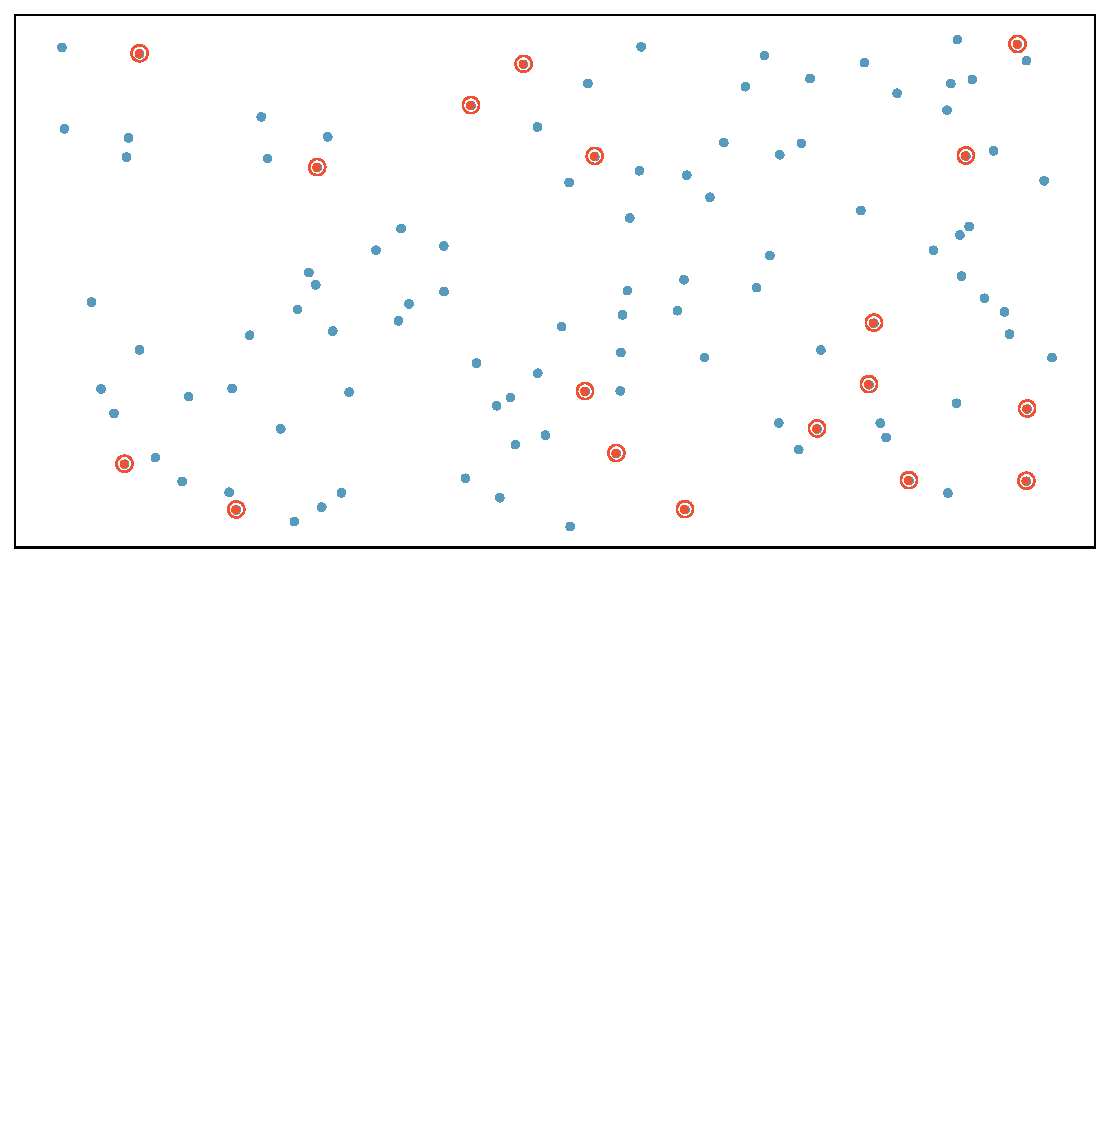
\includegraphics[width=0.9\textwidth]{1-3_sampling_principles_strategies/figures/sampling_methods/simple}
\end{center}

\end{frame}

%%%%%%%%%%%%%%%%%%%%%%%%%%%%%%%%%%%%

\begin{frame}
\frametitle{層化抽出}

\hl{層}は似た観測値からなる。各層から\underline{それぞれ}単純無作為抽出を行う。

\begin{center}
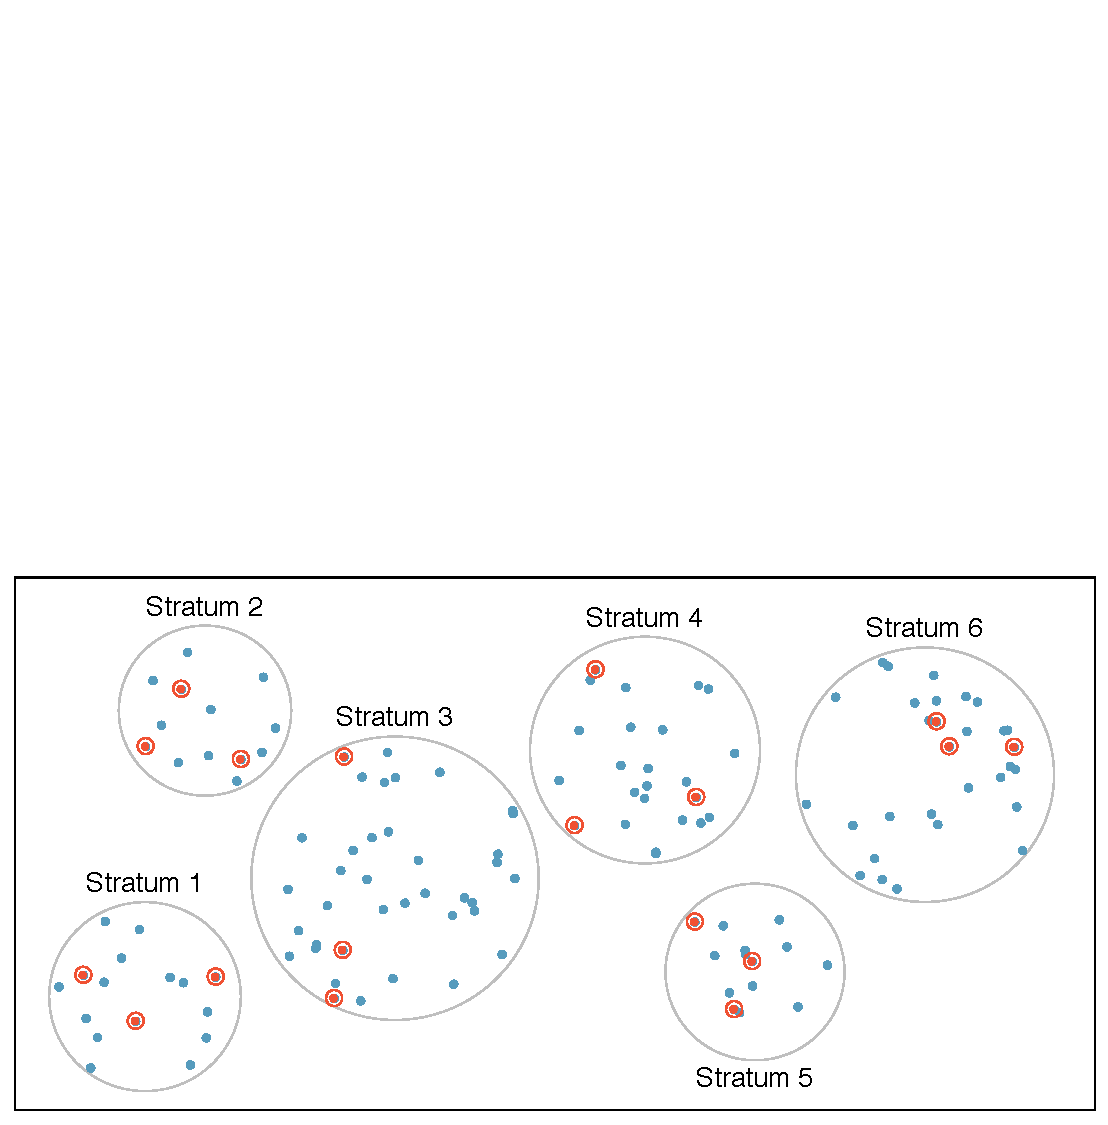
\includegraphics[width=0.9\textwidth]{1-3_sampling_principles_strategies/figures/sampling_methods/stratified}
\end{center}

\end{frame}

%%%%%%%%%%%%%%%%%%%%%%%%%%%%%%%%%%%%

\begin{frame}
\frametitle{クラスター抽出}

\hl{クラスター}は通常、均質な観測値からなるわけではない。
クラスターを単純無作為抽出し、そのクラスター内の\underline{すべて}の観測値を調査する。
経済的な理由から選ばれることが多い。

\begin{center}
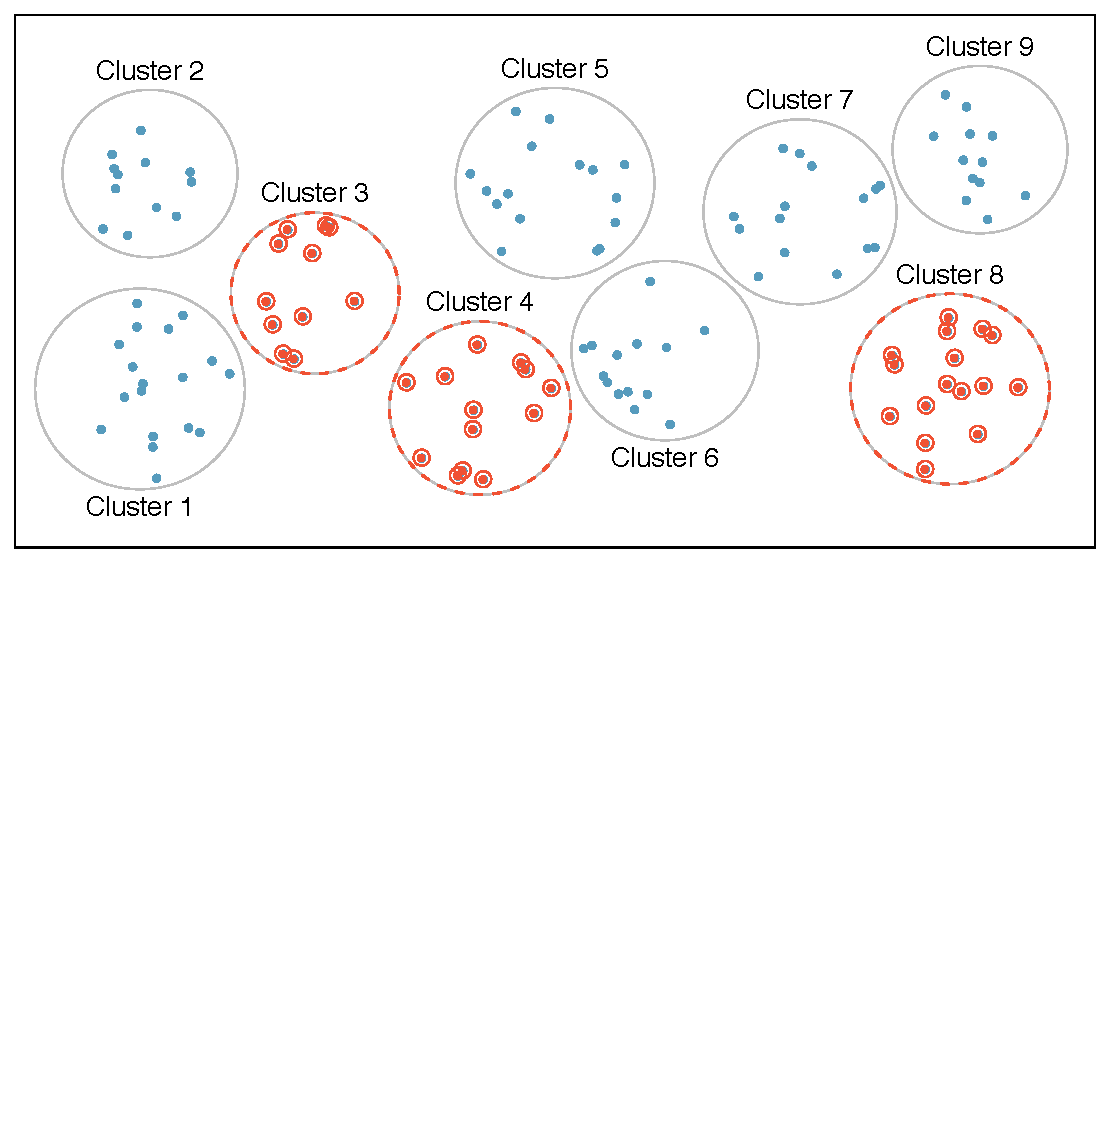
\includegraphics[width=0.9\textwidth]{1-3_sampling_principles_strategies/figures/sampling_methods/cluster}
\end{center}

\end{frame}

%%%%%%%%%%%%%%%%%%%%%%%%%%%%%%%%%%%%

\begin{frame}
\frametitle{多段抽出}

\hl{クラスター}は通常、均質な観測値からなるわけではない。
クラスターを単純無作為抽出し、さらに抽出されたクラスターから観測値を単純無作為抽出する。

\begin{center}
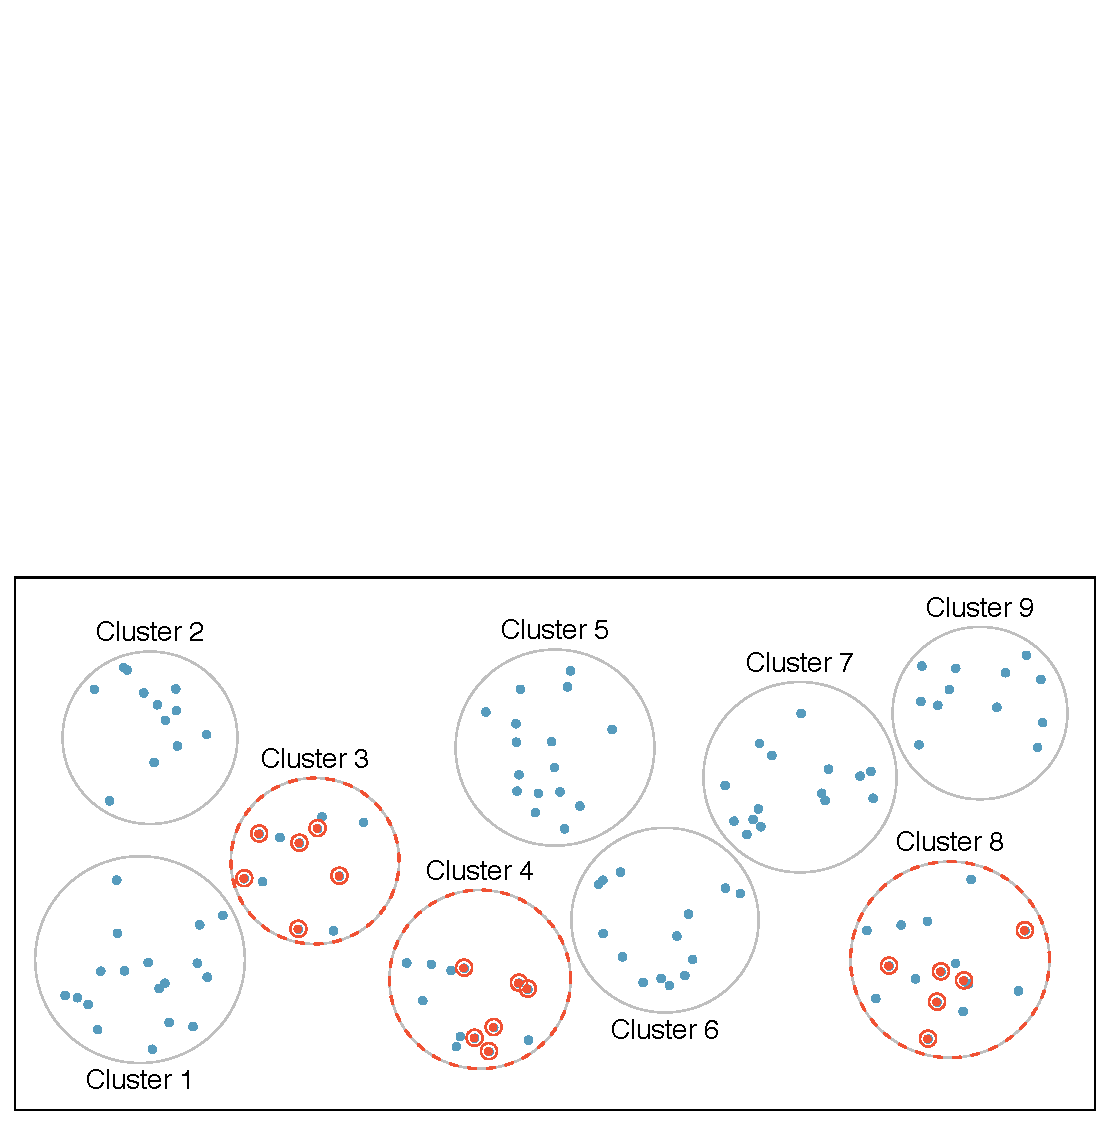
\includegraphics[width=0.9\textwidth]{1-3_sampling_principles_strategies/figures/sampling_methods/multistage}
\end{center}

\end{frame}

%%%%%%%%%%%%%%%%%%%%%%%%%%%%%%%%%%%%

\begin{frame}
\frametitle{練習問題}

\pq{ある市議会が、市の郊外地区で世帯調査を実施するよう要請した。
この地区は多くの異なるユニークな地域（大型住宅が多い地域、アパートだけの地域など）に分かれている。
次のどの方法が\emph{最も}効果的でないか？}

\begin{enumerate}[(a)]
\item 単純無作為抽出
\solnMult{クラスター抽出}
\item 層化抽出
\item ブロックサンプリング
\end{enumerate}

\end{frame}

%%%%%%%%%%%%%%%%%%%%%%%%%%%%%%%%%%%%

%%%%%%%%%%%%%%%%%%%%%%%%%%%%%%%%%%%%

\section{実験}

%%%%%%%%%%%%%%%%%%%%%%%%%%%%%%%%%%%%

\begin{frame}
\frametitle{実験計画の原則}

\begin{enumerate}

\item \hl{統制：}直接研究している変数以外の変数の（潜在的な）影響を統制する。

\item \hl{無作為化：}可能な限り、被験者を処置にランダムに割り当て、
母集団からランダムにサンプリングする。

\item \hl{反復：}研究内では十分に大きな標本を収集することで反復する。
あるいは研究全体を繰り返す。

\item \hl{ブロッキング：}応答変数に影響を与えることが分かっている、
または疑われる変数がある場合、まずその変数に基づいて被験者を
\hl{ブロック}にグループ化し、各ブロック内でケースを処置群にランダムに割り当てる。

\end{enumerate}

\end{frame}

%%%%%%%%%%%%%%%%%%%%%%%%%%%%%%%%%%%%

\begin{frame}
\frametitle{ブロッキングについて詳しく}

\twocol{0.25}{0.75}
{
\begin{center}

\includegraphics[width=\textwidth]{1-4_experiments/figures/gu}
\end{center}
}
{
\begin{itemize}
\item エナジーゲルが走力を向上させるかを調べる実験を設計したい：

\begin{itemize}
\item 処置群：エナジーゲルあり
\item 対照群：エナジーゲルなし
\end{itemize}

\item エナジーゲルがプロとアマチュアのアスリートに異なる影響を与えると疑われるため、
プロかどうかでブロッキングを行う：

\begin{itemize}
\item 標本をプロとアマチュアに分ける
\item プロのアスリートを処置群と対照群にランダムに割り当てる
\item アマチュアのアスリートを処置群と対照群にランダムに割り当てる
\item これにより、処置群と対照群にプロ・アマチュアが均等に代表される
\end{itemize}
\end{itemize}
}

\dq{なぜこれが重要か？ 他にブロッキングすべき変数はあるか？}

\end{frame}

%%%%%%%%%%%%%%%%%%%%%%%%%%%%%%%%%%%%

\begin{frame}
\frametitle{練習問題}

\pq{照明レベルと騒音レベルが学生の試験成績に与える影響を調べる研究を設計する。
研究者は照明と騒音が男女で異なる効果を持つ可能性があると考え、
両性が各グループに均等に含まれるようにしたいと考えている。
次のうち正しいものはどれか？}

\begin{enumerate}[(a)]
\item 説明変数が3つ（照明・騒音・性別）、応答変数が1つ（試験成績）である。
\solnMult{説明変数が2つ（照明と騒音）、ブロッキング変数が1つ（性別）、応答変数が1つ（試験成績）である。}
\item 説明変数が1つ（性別）、応答変数が3つ（照明・騒音・試験成績）である。
\item ブロッキング変数が2つ（照明と騒音）、説明変数が1つ（性別）、応答変数が1つ（試験成績）である。
\end{enumerate}

\end{frame}

%%%%%%%%%%%%%%%%%%%%%%%%%%%%%%%%%%%%

\begin{frame}
\frametitle{ブロッキング変数と説明変数の違い}

\begin{itemize}

\item 要因（factor）とは、実験単位に課すことができる条件のことである。

\item ブロッキング変数とは、実験単位がもともと持っている特性であり、
その影響を統制したいものである。

\item ブロッキングは層化に似ているが、
サンプリングの際ではなく実験設定においてランダムに割り当てる際に用いられる。

\end{itemize}

\end{frame}

%%%%%%%%%%%%%%%%%%%%%%%%%%%%%%%%%%%%

\begin{frame}
\frametitle{実験計画の用語（続き）}

\begin{itemize}

\item \hl{プラセボ：}偽の処置。医学研究では対照群に用いられることが多い。

\item \hl{プラセボ効果：}特別な処置を受けていると信じるだけで、
実験単位が改善を示す現象。

\item \hl{盲検化（ブラインディング）：}実験単位が自分が対照群か処置群かを
知らない状態にすること。

\item \hl{二重盲検：}実験単位と、患者に関わる研究者の両方が、
誰が対照群で誰が処置群かを知らない状態にすること。

\end{itemize}

\end{frame}

%%%%%%%%%%%%%%%%%%%%%%%%%%%%%%%%%%%%

\begin{frame}
\frametitle{練習問題}

\pq{観察研究と実験の主な違いは何か？}

\begin{enumerate}[(a)]
\item 実験は研究室で行われるが、観察研究は必ずしも研究室で行う必要はない。
\item 観察研究では過去に起きたことしか調べられない。
\solnMult{ほとんどの実験では無作為割り当てを用いるが、観察研究では用いない。}
\item 観察研究は、その結果から因果推論ができないため、まったく役に立たない。
\end{enumerate}

\end{frame}

%%%%%%%%%%%%%%%%%%%%%%%%%%%%%%%%%%%%

\begin{frame}
\frametitle{無作為割り当てと無作為抽出}

\begin{center}
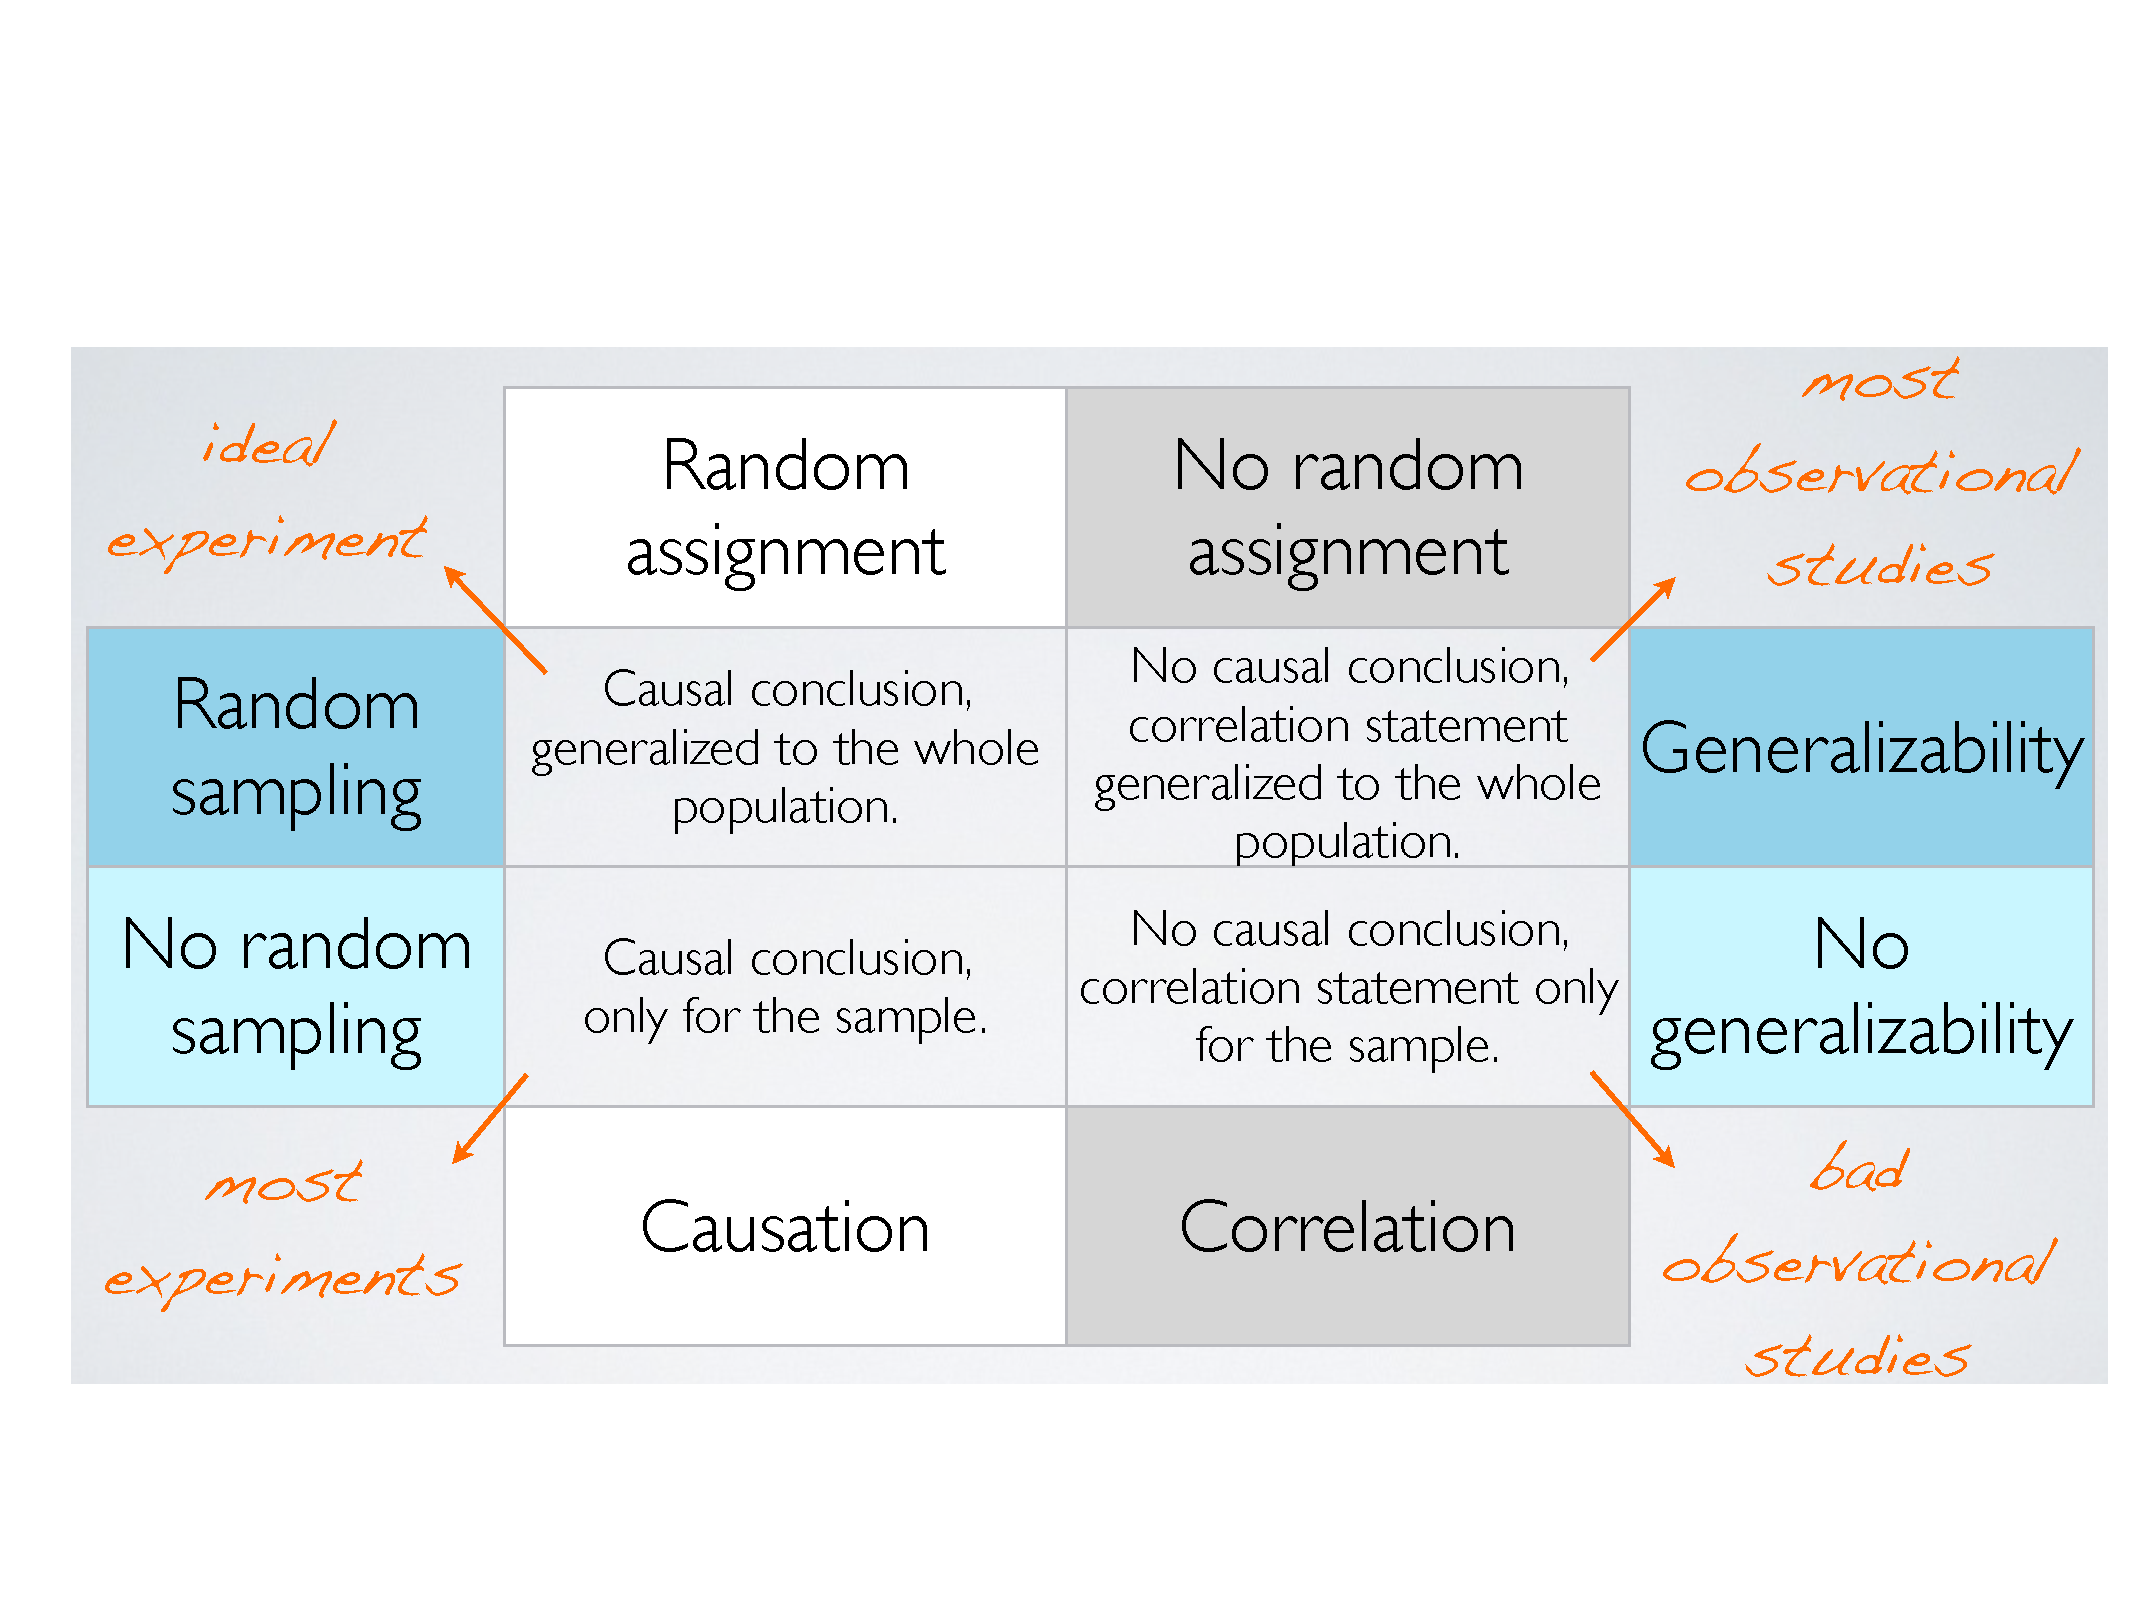
\includegraphics[width=\textwidth]{1-4_experiments/figures/random_sample_assignment}
\end{center}

\end{frame}

%%%%%%%%%%%%%%%%%%%%%%%%%%%%%%%%%%%%



%%%%%%%%%%%%%%%%%%%%%%%%%%%%%%%%%%%%
% ドキュメント終了
%%%%%%%%%%%%%%%%%%%%%%%%%%%%%%%%%%%%

\end{document}
